\documentclass[10pt,twocolumn,letterpaper]{article}
\usepackage[top=0.75in,bottom=1in,left=0.625in,right=0.625in,columnsep=0.25in]{geometry}
\usepackage[T1]{fontenc}
\usepackage[utf8]{inputenc}
\usepackage{mathptmx}
\usepackage[scaled=0.9]{helvet}
\usepackage{courier}
\usepackage{graphicx,amsmath,amssymb,booktabs,array,multirow,url}
\usepackage{tikz}
\usetikzlibrary{arrows.meta,positioning,calc,shapes.geometric,fit}
\usepackage[font=footnotesize,labelsep=period]{caption}
\usepackage{stfloats}
\usepackage{enumitem}
\setlist[itemize]{leftmargin=1.2em,itemsep=1pt,topsep=2pt,parsep=0pt}
\usepackage[hidelinks]{hyperref}
\setlength{\parindent}{1.0em}
\setlength{\parskip}{0pt}
\renewcommand{\baselinestretch}{0.98}
\pagestyle{plain}
\sloppy
\hyphenpenalty=200
\captionsetup[table]{labelformat=simple,labelsep=newline,textfont=sc,font=footnotesize,justification=centering,position=top}
\renewcommand{\thetable}{\Roman{table}}
\renewcommand{\tablename}{TABLE}
\captionsetup[figure]{name={Fig.}}
\makeatletter
\renewcommand\section{\@startsection{section}{1}{\z@}{1.4ex plus .3ex minus .2ex}{1ex plus .1ex}{\centering\normalfont\footnotesize\scshape}}
\renewcommand\subsection{\@startsection{subsection}{2}{\z@}{1.1ex plus .2ex minus .2ex}{0.5ex plus .1ex}{\normalfont\normalsize\itshape}}
\renewcommand\subsubsection{\@startsection{subsubsection}{3}{\parindent}{0.8ex}{-1em}{\normalfont\normalsize\itshape}}
\renewcommand\thesection{\Roman{section}.}
\renewcommand\thesubsection{\Alph{subsection}.}
\renewcommand\thesubsubsection{\arabic{subsubsection})}
\renewcommand{\@seccntformat}[1]{\csname the#1\endcsname\hspace{0.5em}}
\makeatother
\newcommand{\sys}{\textsc{CrossState}}
\newcommand{\code}[1]{\texttt{\small #1}}
\setlength{\textfloatsep}{8pt plus 2pt minus 2pt}
\setlength{\floatsep}{8pt plus 2pt minus 2pt}
\setlength{\intextsep}{8pt plus 2pt minus 2pt}

\begin{document}

\title{\vspace{-0.5em}\fontsize{21}{23}\selectfont \sys: Verified Cross-Target Migration of Stateful TCP Firewall State Between P4/BMv2 and eBPF/XDP Data Planes\vspace{-0.3em}}

\author{%
\begin{tabular}[t]{c@{\hspace{3em}}c}
\large Srijan Raghavula & \large Karthik Alakanti\\
\small Roll No.\ 23BCS102 & \small Roll No.\ 23BCS009\\
\end{tabular}\\[0.8ex]
\small Supervisor: Dr.\ Jagadeesha R.\ Bhatt\\
\small Department of Computer Science and Engineering\\
\small Indian Institute of Information Technology Dharwad, Karnataka, India%
}
\date{}
\maketitle
\thispagestyle{plain}

\begin{abstract}
\noindent\textbf{\textit{Abstract}---}Stateful network functions keep per-flow state inside the data plane, so moving a function between heterogeneous targets normally breaks established connections. This report presents \sys, a framework that migrates TCP connection-tracking state between a P4\textsubscript{16} firewall on the BMv2 software switch and an eBPF/XDP firewall, in both directions. \sys\ defines one logical state schema with a deterministic CRC32 slot mapping, and a quiesced checkpoint protocol with a fail-closed readiness gate, per-record read-back, rollback, a source-stability check and an audit record. We evaluate five research questions on 1{,}000 synthetic flows and on 1{,}000 complete flows (18{,}944 packets) from a MAWI trace. Four alternating migrations all pass; the final 1{,}086-record tables are identical; all 18{,}944 live decisions match a reference model; and a 100{,}000-packet randomized differential test shows no mismatch. Replaying the same packets through the reference model without migration drops 99.7\% of the 17{,}944 post-cutover packets and disrupts 996 of 1{,}000 flows, whereas migration drops none. Writing only changed records cuts record writes by 40\% over rewriting the whole table, and a collision study shows that the direct-mapped 65{,}536-slot table rejects 0.85\% of new flows at 1{,}000 flows and 7.2\% at 10{,}000, which bounds practical capacity. The evaluation is of correctness under quiesced operation; no line-rate claims are made.
\end{abstract}

\begin{center}
\small\textbf{\textit{Index Terms}---}\textit{P4, BMv2, eBPF, XDP, stateful firewall, connection tracking, state migration, data-plane portability, MAWI.}
\end{center}

%==========================================================
\section{Introduction}
Security functions are increasingly implemented directly in programmable data planes. P4 \cite{p4} describes protocol-independent pipelines, while eBPF/XDP \cite{xdp} runs packet programs at the earliest point of the Linux receive path, and SmartNICs combine both styles in one device \cite{smartnic}. A connection-tracking firewall is a typical stateful function: it admits inbound packets only if they belong to a connection initiated from the protected side, and so keeps a TCP state and counters per flow \cite{p4sec}.

This state makes the function hard to move. If a firewall is shifted from one target to another for maintenance, rebalancing or recovery, the destination starts with an empty table and established connections look unsolicited. State-management systems address this for software NFs \cite{opennf,splitmerge}, for programmable switches \cite{swing,redplane}, and increasingly for hybrid switch/server or SmartNIC/CPU deployments \cite{switchnic,cora}, but they assume the same NF implementation on both sides. Moving the \emph{same logical state} between a P4 pipeline and an eBPF program, with evidence that nothing was lost or altered, is not addressed.

We study this problem through five research questions:
\begin{itemize}
\item \textbf{RQ1 (Correctness).} Is logical state preserved exactly, and are decisions after cutover identical?
\item \textbf{RQ2 (Necessity).} What happens to traffic if state is not migrated?
\item \textbf{RQ3 (Capacity).} How does the hash-indexed table behave as load grows?
\item \textbf{RQ4 (Cost).} What does a checkpoint write and how long does it take?
\item \textbf{RQ5 (Assurance).} Which mechanisms make a bad transfer detectable or harmless?
\end{itemize}

The contributions are: (i) a target-neutral state schema and a formal equivalence definition (Section~III); (ii) a checkpoint protocol with a fail-closed readiness gate, read-back verification, rollback and an audit trail (Section~IV); (iii) a layered validation ladder from unit tests to real-traffic migration (Section~V); and (iv) an evaluation answering RQ1--RQ5 with a no-migration baseline, a delta-versus-full comparison, a collision study and a cost analysis (Sections~VI--VII).

%==========================================================
\section{Background and Related Work}
\subsection{Stateful Data Planes}
P4 keeps cross-packet state in register arrays; XDP keeps it in BPF maps readable from user space. Recent work extends what stateful P4 pipelines can express \cite{rapid} and combines the two worlds, for example by running eBPF inside a P4 pipeline to allow runtime updates \cite{ebpfp4}. Surveys of programmable security functions note that stateful filters in switches commonly rely on hashed flow identifiers and need extra mechanisms to handle hash collisions \cite{p4sec,cofilter}. BMv2 \cite{bmv2} is the reference P4 target and exposes its registers through a runtime command interface; this is the access path \sys\ uses.

\subsection{State Migration and Replication}
OpenNF \cite{opennf} coordinates NF state movement with forwarding changes to give loss-free and order-preserving guarantees; Split/Merge \cite{splitmerge} partitions flow state for elastic scaling; Swing State \cite{swing} moves register state between programmable switches; RedPlane \cite{redplane} adds a replicated state store and recovery for in-switch applications. For hybrid platforms, Cora \cite{cora} offloads stateful applications to SmartNICs and uses a flow-migration protocol to stay consistent when moving flows between NIC and CPU, and SwitchNIC \cite{switchnic} maintains consistent shared state between a switch and a server. On the theory side, Patowary et al.\ \cite{patowary} study what correct flow migration means across NF instances and show that no criterion stronger than a weak order property can be kept by a system that neither buffers nor drops packets and eventually synchronises. In-band state migration is also used for mobility handling in P4 edge networks \cite{mafaf}.

Table~\ref{tab:related} compares these with \sys. Our position differs in two ways: the unit of migration is a \emph{schema} rather than an implementation, so it works across P4 and eBPF; and every transfer is verified by construction (exact equivalence, stability, audit) rather than assumed. The price is that \sys\ is quiesced, which the first four systems in the table avoid by coordinating with live traffic.

\begin{table}[!t]
\caption{Comparison With Related Work}
\label{tab:related}
\centering\footnotesize
\setlength{\tabcolsep}{2.5pt}
\renewcommand{\arraystretch}{1.05}
\begin{tabular}{@{}p{1.45cm}p{0.65cm}p{2.0cm}p{2.9cm}@{}}
\toprule
\textbf{System} & \textbf{Year} & \textbf{Platforms} & \textbf{Mechanism / guarantee}\\
\midrule
OpenNF \cite{opennf} & 2014 & software NFs & coordinated move; loss-free, order-preserving\\
Swing State \cite{swing} & 2017 & P4 switches & in-band state transfer; consistent updates\\
RedPlane \cite{redplane} & 2021 & Tofino switches & replicated state store; fault tolerance\\
Cora \cite{cora} & 2024 & SmartNIC$\leftrightarrow$CPU & flow-migration protocol; consistency\\
SwitchNIC \cite{switchnic} & 2025 & switch + server & consistent shared state\\
\midrule
\textbf{\sys} & 2026 & BMv2 (P4) $\leftrightarrow$ XDP (eBPF) & schema-level, quiesced; exact equivalence, audit\\
\bottomrule
\end{tabular}
\end{table}

%==========================================================
\section{Problem Formulation}
\subsection{State Model}
Let $N$ be the number of slots. A \emph{flow key} $k=(a,p_a,b,p_b,\pi)$ is the canonicalised 5-tuple (endpoints ordered by address, then port), so both directions of a connection map to one record. A \emph{record} is $r=(k,\sigma,t,c_p,c_b)$ with tracker state $\sigma\in\{\textsc{New},\textsc{Est},\textsc{Closed}\}$, last-seen time $t$, and packet and byte counters $c_p,c_b$ (64-bit, wrapping). The slot of a key is $h(k)=\mathrm{CRC32}(\mathrm{bytes}(k))\bmod N$ over the 13-byte network-order key. A target's table is a partial map $S:\{0,\dots,N-1\}\rightharpoonup R$.

\textbf{Definition 1 (logical equivalence).} Tables $S_A$ and $S_B$ are equivalent, $S_A\equiv S_B$, iff they have the same domain and $S_A(s)=S_B(s)$ for every slot, comparing the decoded tuple $(k,\sigma,t,c_p,c_b)$ rather than the physical encoding (P4 registers versus a BPF map value).

\textbf{Definition 2 (policy step).} Both targets implement the same deterministic function $\delta(S,e)\to(S',d)$ that maps a table and a packet event $e$ to a new table and a decision $d\in\{\textsc{Allow},\textsc{Drop}\}$. Records idle longer than $T=30$~s are treated as absent (lazy expiry); a live record whose key differs from the packet's key is a collision and the packet is dropped.

\textbf{Proposition 1.} If $S_A\equiv S_B$ and both targets implement $\delta$ with the same clock, then for any packet sequence they produce identical decisions and remain equivalent.
\emph{Argument:} $\delta$ is a function of $(S,e)$ only, so identical inputs yield identical outputs by induction on the sequence. The proposition shows why exact equivalence is the right goal. It does not cover packets that arrive \emph{during} a transfer, which is why \sys\ is quiesced.

\subsection{Objectives}
The migration problem is: given $S_A$ at the source, produce a destination table $S_B\equiv S_A$ and certify it, so that Proposition~1 applies. The certificate must fail if the transfer is partial, if any record is altered, or if the source changed while it was being read.

%==========================================================
\section{Design}
\subsection{Architecture}
Fig.~\ref{fig:arch} shows the system. A replay harness injects packets into either target through a shim header. A checkpoint controller reads each table, compares it, and writes missing or changed records to the destination. A Python reference model processes the same packets and supplies expected decisions and final state.

\begin{figure*}[!t]
\centering
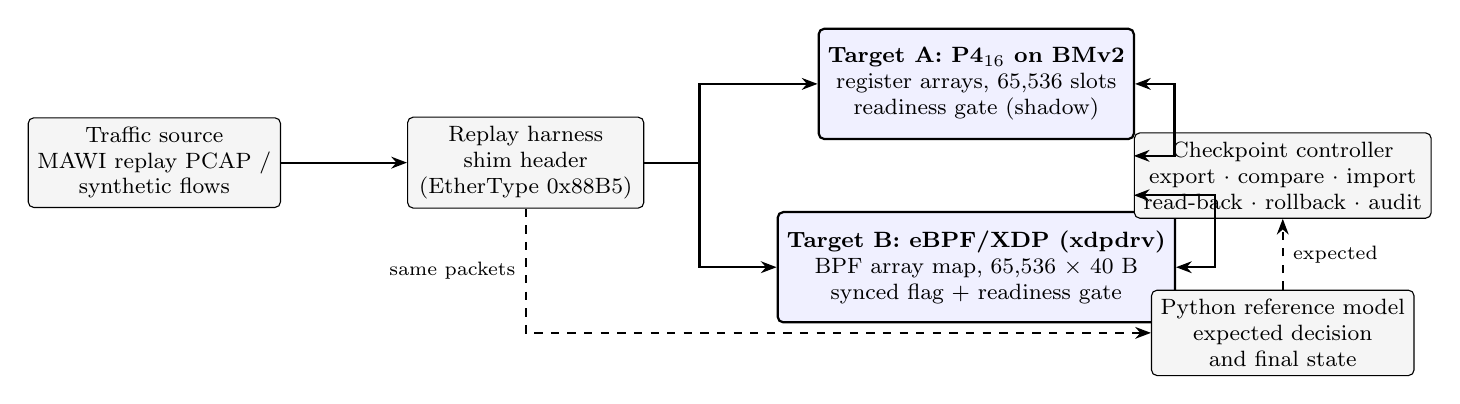
\begin{tikzpicture}[
  node distance=1.0cm and 1.6cm,
  box/.style={draw,rounded corners=2pt,align=center,minimum height=1.0cm,minimum width=3.0cm,font=\footnotesize,fill=gray!8},
  tgt/.style={draw,thick,rounded corners=2pt,align=center,minimum height=1.4cm,minimum width=3.9cm,font=\footnotesize,fill=blue!6},
  ar/.style={-{Stealth[length=2mm]},thick},
  dar/.style={{Stealth[length=2mm]}-{Stealth[length=2mm]},thick}]
\node[box] (traffic) {Traffic source\\ MAWI replay PCAP /\\ synthetic flows};
\node[box,right=of traffic] (shim) {Replay harness\\ shim header\\ (EtherType 0x88B5)};
\node[tgt,right=2.2cm of shim,yshift=1.0cm] (bmv2) {\textbf{Target A: P4$_{16}$ on BMv2}\\ register arrays, 65{,}536 slots\\ readiness gate (shadow)};
\node[tgt,below=0.9cm of bmv2] (xdp) {\textbf{Target B: eBPF/XDP (xdpdrv)}\\ BPF array map, 65{,}536 $\times$ 40 B\\ synced flag + readiness gate};
\node[box,minimum width=3.7cm,right=2.0cm of $(bmv2)!0.5!(xdp)$] (ctl) {Checkpoint controller\\ export $\cdot$ compare $\cdot$ import\\ read-back $\cdot$ rollback $\cdot$ audit};
\node[box,below=0.9cm of ctl] (ref) {Python reference model\\ expected decision\\ and final state};
\draw[ar] (traffic) -- (shim);
\draw[ar] (shim.east) -- ++(0.7,0) |- (bmv2.west);
\draw[ar] (shim.east) -- ++(0.7,0) |- (xdp.west);
\draw[dar] (bmv2.east) -- ++(0.5,0) |- ($(ctl.west)+(0,0.25)$);
\draw[dar] (xdp.east) -- ++(0.5,0) |- ($(ctl.west)+(0,-0.25)$);
\draw[ar,dashed] (shim.south) |- (ref.west) node[pos=0.25,left,font=\scriptsize] {same packets};
\draw[ar,dashed] (ref.north) -- (ctl.south) node[midway,right,font=\scriptsize] {expected};
\end{tikzpicture}
\caption{\sys\ architecture. The controller moves logical state in either direction; the reference model supplies expected decisions and final state.}
\label{fig:arch}
\end{figure*}

\subsection{Specification and Policy}
All parameters are generated from one machine-readable specification (Table~\ref{tab:spec}) into constants for both targets, so the two programs cannot drift apart. The policy follows $\delta$: an inside SYN creates \textsc{New}; a reverse SYN-ACK moves \textsc{New} to \textsc{Est}; FIN or RST moves to \textsc{Closed}; a reverse packet before SYN-ACK, a packet with no live state, and a packet after \textsc{Closed} are dropped (an inside SYN reopens a closed flow). The eBPF build used here runs in \emph{test-echo} mode: its decision is returned in the shim flags and recorded, but the packet is not dropped on the wire, so enforcement in the data path is not part of this evaluation.

\begin{table}[!t]
\caption{Specification Parameters}
\label{tab:spec}
\centering\footnotesize
\begin{tabular}{@{}ll@{}}
\toprule
\textbf{Parameter} & \textbf{Value}\\
\midrule
Slots $N$ & 65{,}536 (direct-mapped)\\
Flow key & canonical 5-tuple, 13 B\\
Slot hash & CRC32(key) mod $N$\\
Idle timeout $T$ & 30 s, lazy expiry\\
Counters & 64-bit, wrap modulo $2^{64}$\\
Collision policy & reject (live mismatch $\rightarrow$ DROP)\\
XDP record / map size & 40 B / 2.6 MB (array map)\\
Shim header & EtherType 0x88B5; 6 B time, 4 B id, 1 B dir.\\
Targets & BMv2 \texttt{simple\_switch}; XDP \texttt{xdpdrv} on veth\\
\bottomrule
\end{tabular}
\end{table}

\subsection{Checkpoint Protocol}
A checkpoint runs in one direction with an explicit quiescence acknowledgement (Fig.~\ref{fig:proto}). Three mechanisms provide the assurance asked for in RQ5. \emph{Fail-closed readiness gate:} imported records are written with the synced flag cleared, and the destination is marked ready only after exact equivalence is verified; an unsynced shadow update is skipped by the eBPF program. \emph{Read-back and rollback:} each written record is read back, and a best-effort rollback of the slot is attempted if a write fails. \emph{Source stability:} the source is exported twice and the two exports must be equivalent, because BMv2 register reads are not an atomic snapshot. Each checkpoint retains ten artefacts and an audit JSON.

\begin{figure}[!t]
\centering
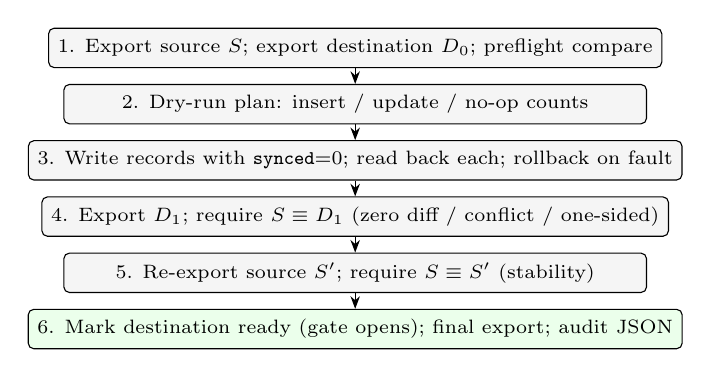
\begin{tikzpicture}[
  s/.style={draw,rounded corners=2pt,align=center,font=\scriptsize,minimum width=7.4cm,minimum height=0.5cm,fill=gray!8},
  g/.style={draw,rounded corners=2pt,align=center,font=\scriptsize,minimum width=7.4cm,minimum height=0.5cm,fill=green!8},
  ar/.style={-{Stealth[length=1.6mm]}}]
\node[s] (a) {1. Export source $S$; export destination $D_0$; preflight compare};
\node[s,below=0.2cm of a] (b) {2. Dry-run plan: insert / update / no-op counts};
\node[s,below=0.2cm of b] (c) {3. Write records with \texttt{synced}=0; read back each; rollback on fault};
\node[s,below=0.2cm of c] (d) {4. Export $D_1$; require $S\equiv D_1$ (zero diff / conflict / one-sided)};
\node[s,below=0.2cm of d] (e) {5. Re-export source $S'$; require $S\equiv S'$ (stability)};
\node[g,below=0.2cm of e] (f) {6. Mark destination ready (gate opens); final export; audit JSON};
\foreach \x/\y in {a/b,b/c,c/d,d/e,e/f}{\draw[ar] (\x) -- (\y);}
\end{tikzpicture}
\caption{Checkpoint protocol. Any failed check aborts before the readiness gate opens.}
\label{fig:proto}
\end{figure}

%==========================================================
\section{Implementation and Validation Ladder}
\subsection{Implementation}
The P4 firewall runs on BMv2 \texttt{simple\_switch} and is accessed through its runtime command interface, one command subprocess per record; the XDP firewall is loaded in driver mode on a veth interface and its map is accessed with \texttt{bpftool}. Export, import, comparison and audit are Python tools sharing one snapshot format. All experiments ran on a single Linux host (a WSL2-based environment). Both targets are software.

\subsection{Validation Ladder}
Correctness is checked in layers of increasing realism (Table~\ref{tab:ladder}). The differential test (G2) drives 100{,}000 randomized packets over 64 flows through XDP and the reference model and compares every decision and 64 touched slots; it reports no missing or duplicate packets and no mismatch, in 72.9~s. Its own record notes that it validates decision observation, not production enforcement.

\begin{table}[!t]
\caption{Validation Ladder}
\label{tab:ladder}
\centering\footnotesize
\setlength{\tabcolsep}{2.5pt}
\begin{tabular}{@{}llr@{}}
\toprule
\textbf{Level} & \textbf{What is checked} & \textbf{Result}\\
\midrule
Unit tests & spec, codegen, export/import, sync & 67 pass\\
G1 & BMv2 vs.\ oracle, 5 traces (new, establish, & 20/20\\
 & close/reopen, expiry, collision) & \\
G3 & BMv2 CRC slot and record vs.\ vectors & 20/20\\
G2 & XDP vs.\ reference, 100{,}000 random pkts & 0 mismatch\\
E1 & 1{,}000 synthetic flows, 4 checkpoints & pass\\
E2 & 1{,}000 MAWI flows, 4 checkpoints & pass\\
E4 & 7 labelled ALLOW/DROP controls $\times$ 2 targets & 14/14\\
\bottomrule
\end{tabular}
\end{table}

%==========================================================
\section{Experimental Methodology}
\subsection{Workloads}
\textbf{E1 (synthetic).} 1{,}000 flows to \code{10.201.0.1:443}, two groups of 500, each sending a SYN and an ACK (40~B packets). \textbf{E2 (MAWI).} The workload derives from the MAWI Samplepoint-F capture of 6~August 2024 \cite{mawi}: 201{,}918{,}230 frames, 50{,}526{,}462 IPv4/TCP packets, 900.4~s. A preprocessing pass tracked 63{,}295 candidate flows and selected 1{,}000 complete bidirectional handshakes (30~s idle limit, 1{,}000-packet cap, truncation at first FIN/RST); 23 candidates were rejected for slot collisions with the 1{,}086 occupied slots. The replay PCAP holds 18{,}944 packets (973{,}852 IP bytes); the captured initiator is the \emph{inside} endpoint. \textbf{E3} is a 20-flow, 301-packet subset; \textbf{E4} is seven labelled control packets (Table~\ref{tab:exp}).

\subsection{Migration Schedule}
Flows are split into Cohort~A and B of 500. (1)~A SYNs on BMv2; (2)~checkpoint~1 BMv2$\to$XDP; (3)~A follow-up packets on XDP; (4)~checkpoint~2 XDP$\to$BMv2; (5)~B SYNs on XDP; (6)~checkpoint~3 XDP$\to$BMv2; (7)~B follow-up on BMv2; (8)~checkpoint~4 BMv2$\to$XDP. Each flow is created on one target and finished on the other, so a correct decision on a follow-up packet requires that its state was migrated. All runs start from an 86-record baseline.

\subsection{Baselines and Studies}
\begin{itemize}
\item \textbf{No-migration baseline (RQ2).} The same 18{,}944 packets are replayed through the reference model under the same schedule, but each checkpoint copies nothing, so the destination starts empty. This is a model-based baseline; the live targets were not run in this mode. As a consistency check, the \emph{migrated} replay through the model reproduces the live result exactly.
\item \textbf{Collision study (RQ3).} Random canonical keys are inserted using the project's own slot function with the reject policy; 30 trials per load from 100 to 65{,}536 flows.
\item \textbf{Delta versus full write (RQ4).} The records written per checkpoint by the tool (changed records only) are compared with the count if every source record were rewritten.
\end{itemize}

\subsection{Metrics}
(a) Decision agreement with the reference model; (b) exact-match records between targets and against the reference; (c) checkpoint pass/fail and record counts; (d) dropped packets and disrupted flows; (e) rejected-flow percentage; (f) records written and elapsed time per checkpoint. Elapsed time is wall-clock for the whole tool run (exports, comparison, writes, read-back), not data-plane latency.

\begin{table}[!t]
\caption{Experiments and MAWI Workload}
\label{tab:exp}
\centering\footnotesize
\setlength{\tabcolsep}{3pt}
\begin{tabular}{@{}lllrr@{}}
\toprule
\textbf{ID} & \textbf{Workload} & \textbf{Mode} & \textbf{Flows} & \textbf{Pkts}\\
\midrule
E1 & Synthetic & live, 4 ckpts & 1{,}000 & 2{,}000\\
E2 & MAWI full & live, 4 ckpts & 1{,}000 & 18{,}944\\
E3 & MAWI subset & live, 4 ckpts & 20 & 301\\
E4 & Controls & live & 7 & 14\\
\midrule
\multicolumn{5}{@{}l}{MAWI E2: packets/flow mean 18.9, median 8, min 4, max 1{,}000;}\\
\multicolumn{5}{@{}l}{775 flows end with FIN, 83 with RST, 142 stay established.}\\
\bottomrule
\end{tabular}
\end{table}

%==========================================================
\section{Results}
\subsection{Workload Characteristics}
Flows are short and heavy-tailed (Fig.~\ref{fig:ecdf}): the median has 8 packets while one reaches the 1{,}000 cap. Of the 1{,}000 flows, 858 end \textsc{Closed} and 142 remain \textsc{Established}.

\begin{figure}[!t]
\centering
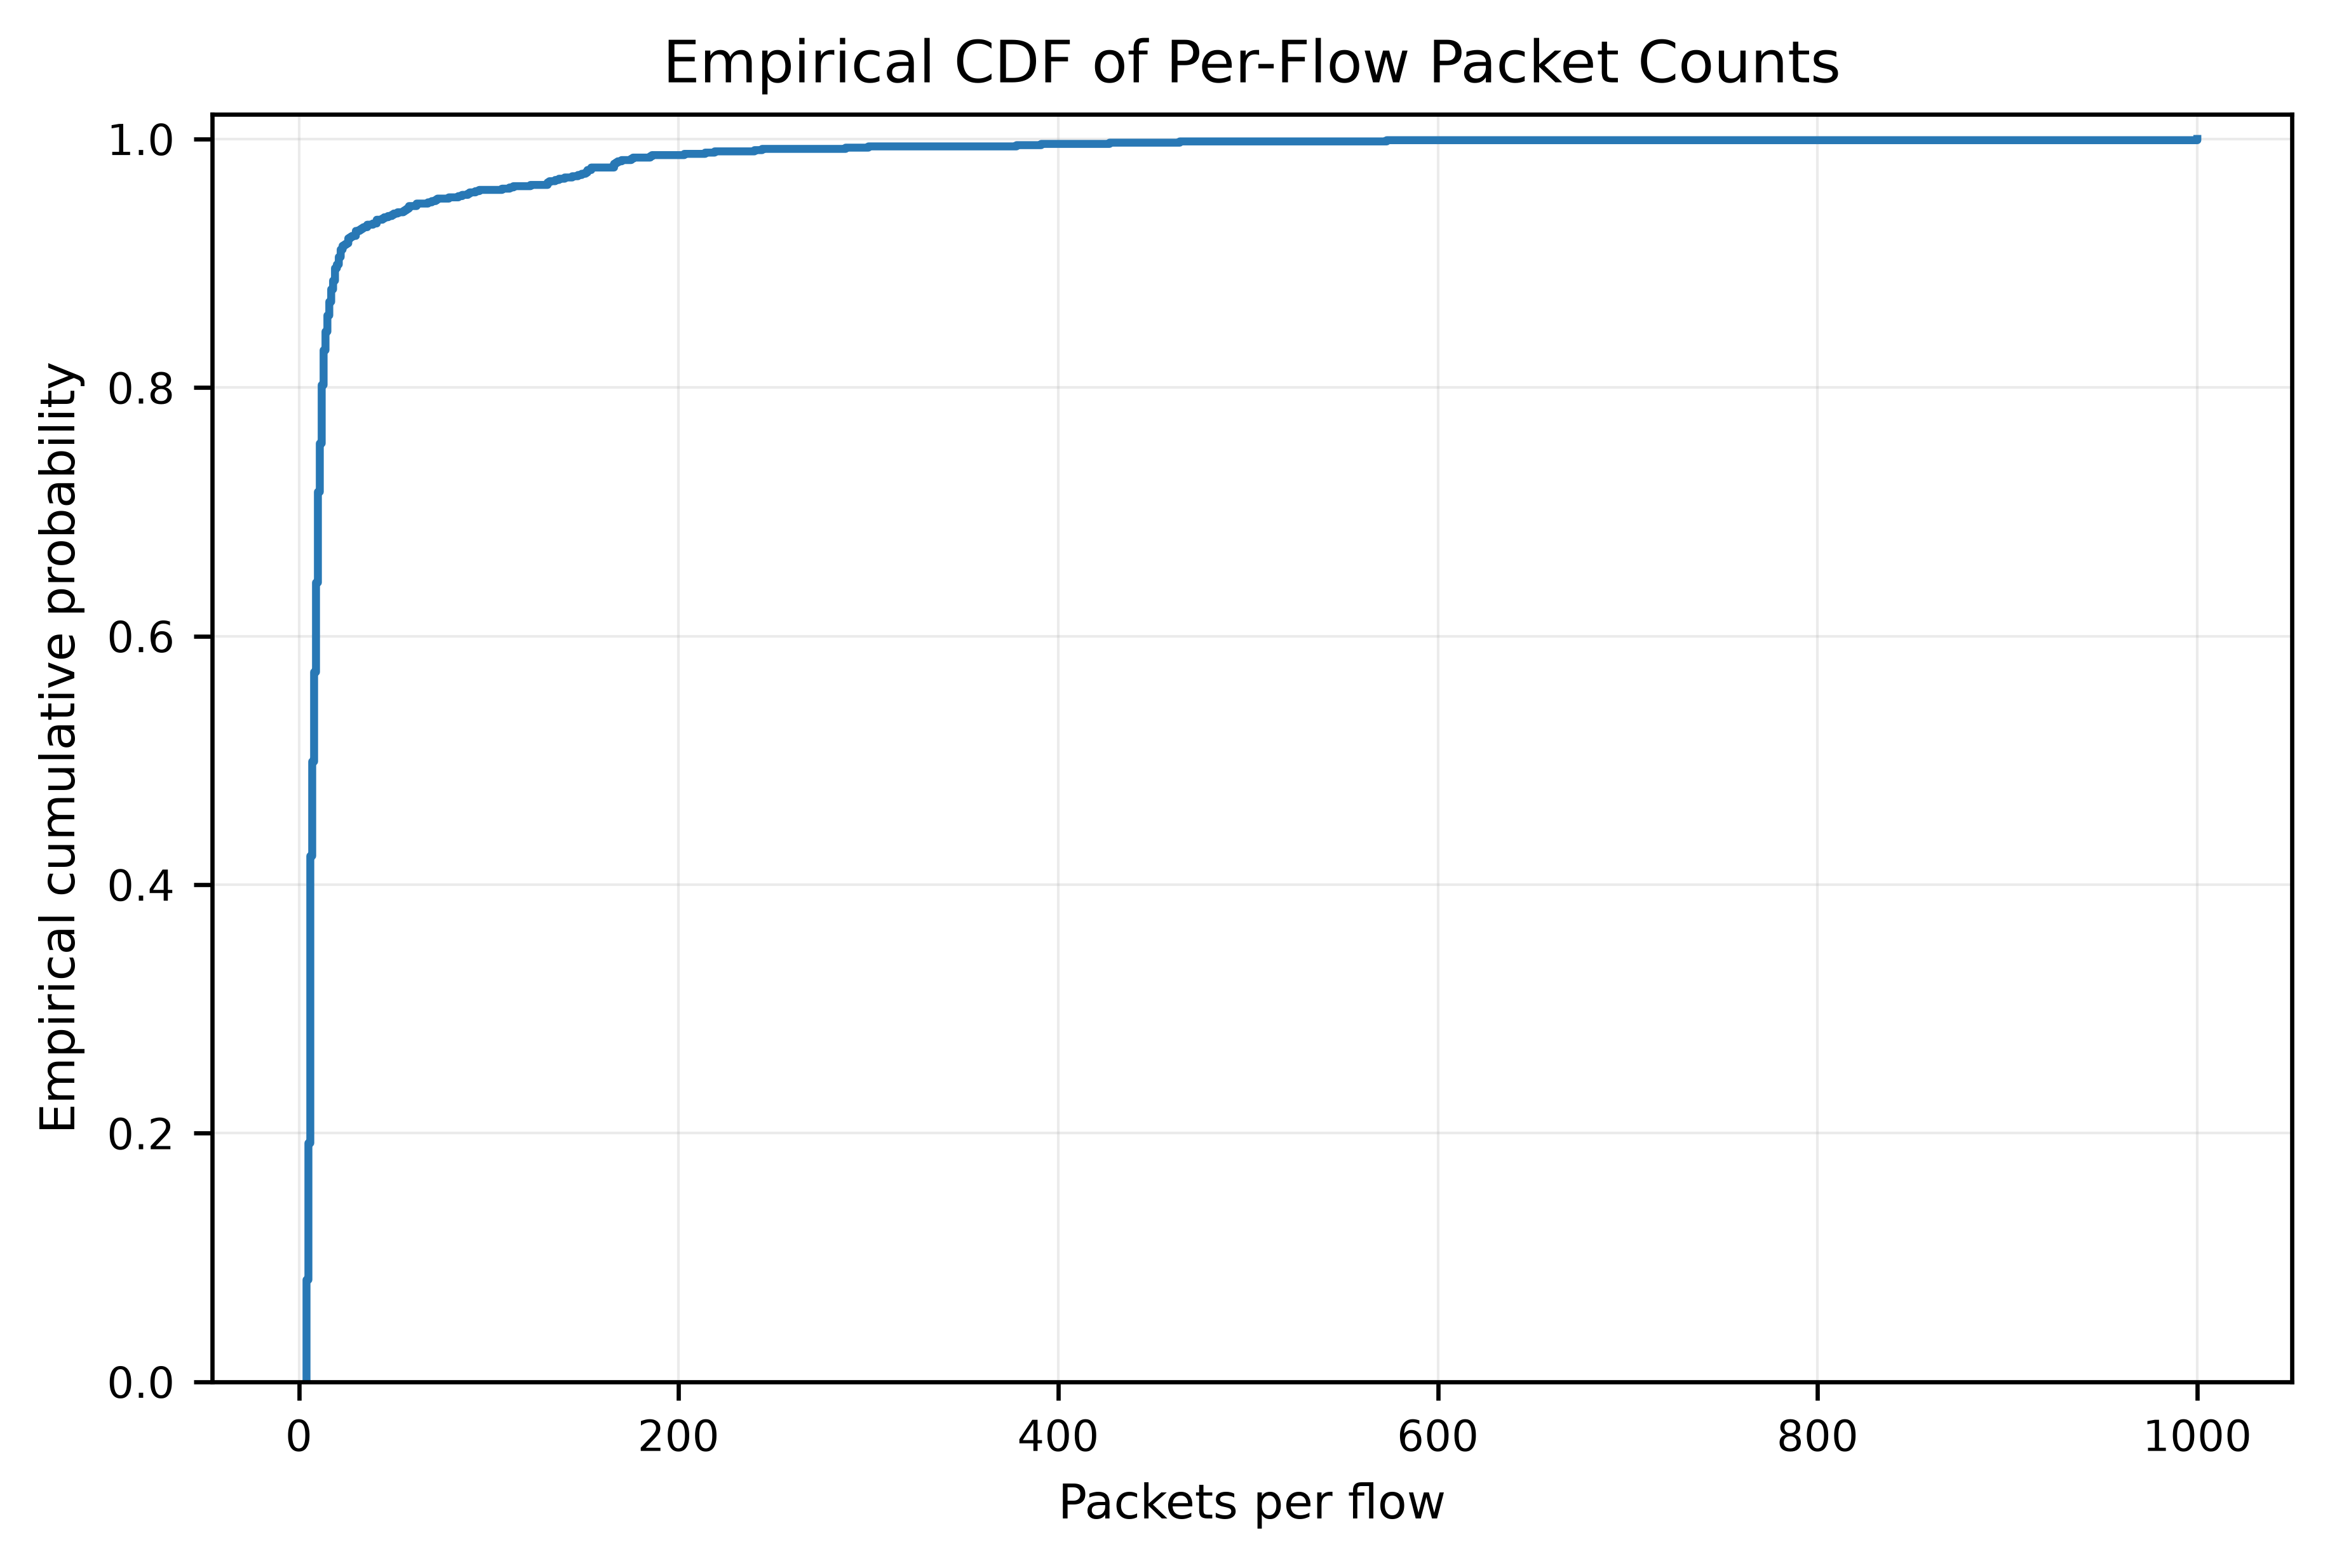
\includegraphics[width=0.92\columnwidth]{figs/mawi_ecdf.png}
\caption{Empirical CDF of packets per selected MAWI flow.}
\label{fig:ecdf}
\end{figure}

\subsection{RQ1: Correctness}
\textbf{State.} Fig.~\ref{fig:stage} shows valid records during E1. BMv2 holds 586 after Cohort~A SYNs while XDP holds 86; checkpoint~1 brings XDP to 586; Cohort~B SYNs raise XDP to 1{,}086 while BMv2 stays at 586; checkpoint~3 closes the gap. The curves coincide after every checkpoint. In E1 and E2 the final tables hold 1{,}086 records each, all exact matches, with no differing, conflicting or one-sided slots (Table~\ref{tab:equiv}); in E2 no migrated flow differs from the reference final state, and packet and byte counters are identical on both targets for every flow. \textbf{Decisions.} All 18{,}944 live decisions in E2 matched the reference model (500 + 7{,}161 + 500 + 10{,}783 across the four phases), 301/301 in E3, and 14/14 for the labelled controls, which supply the DROP cases that legitimate MAWI flows do not.

\begin{figure*}[!t]
\centering
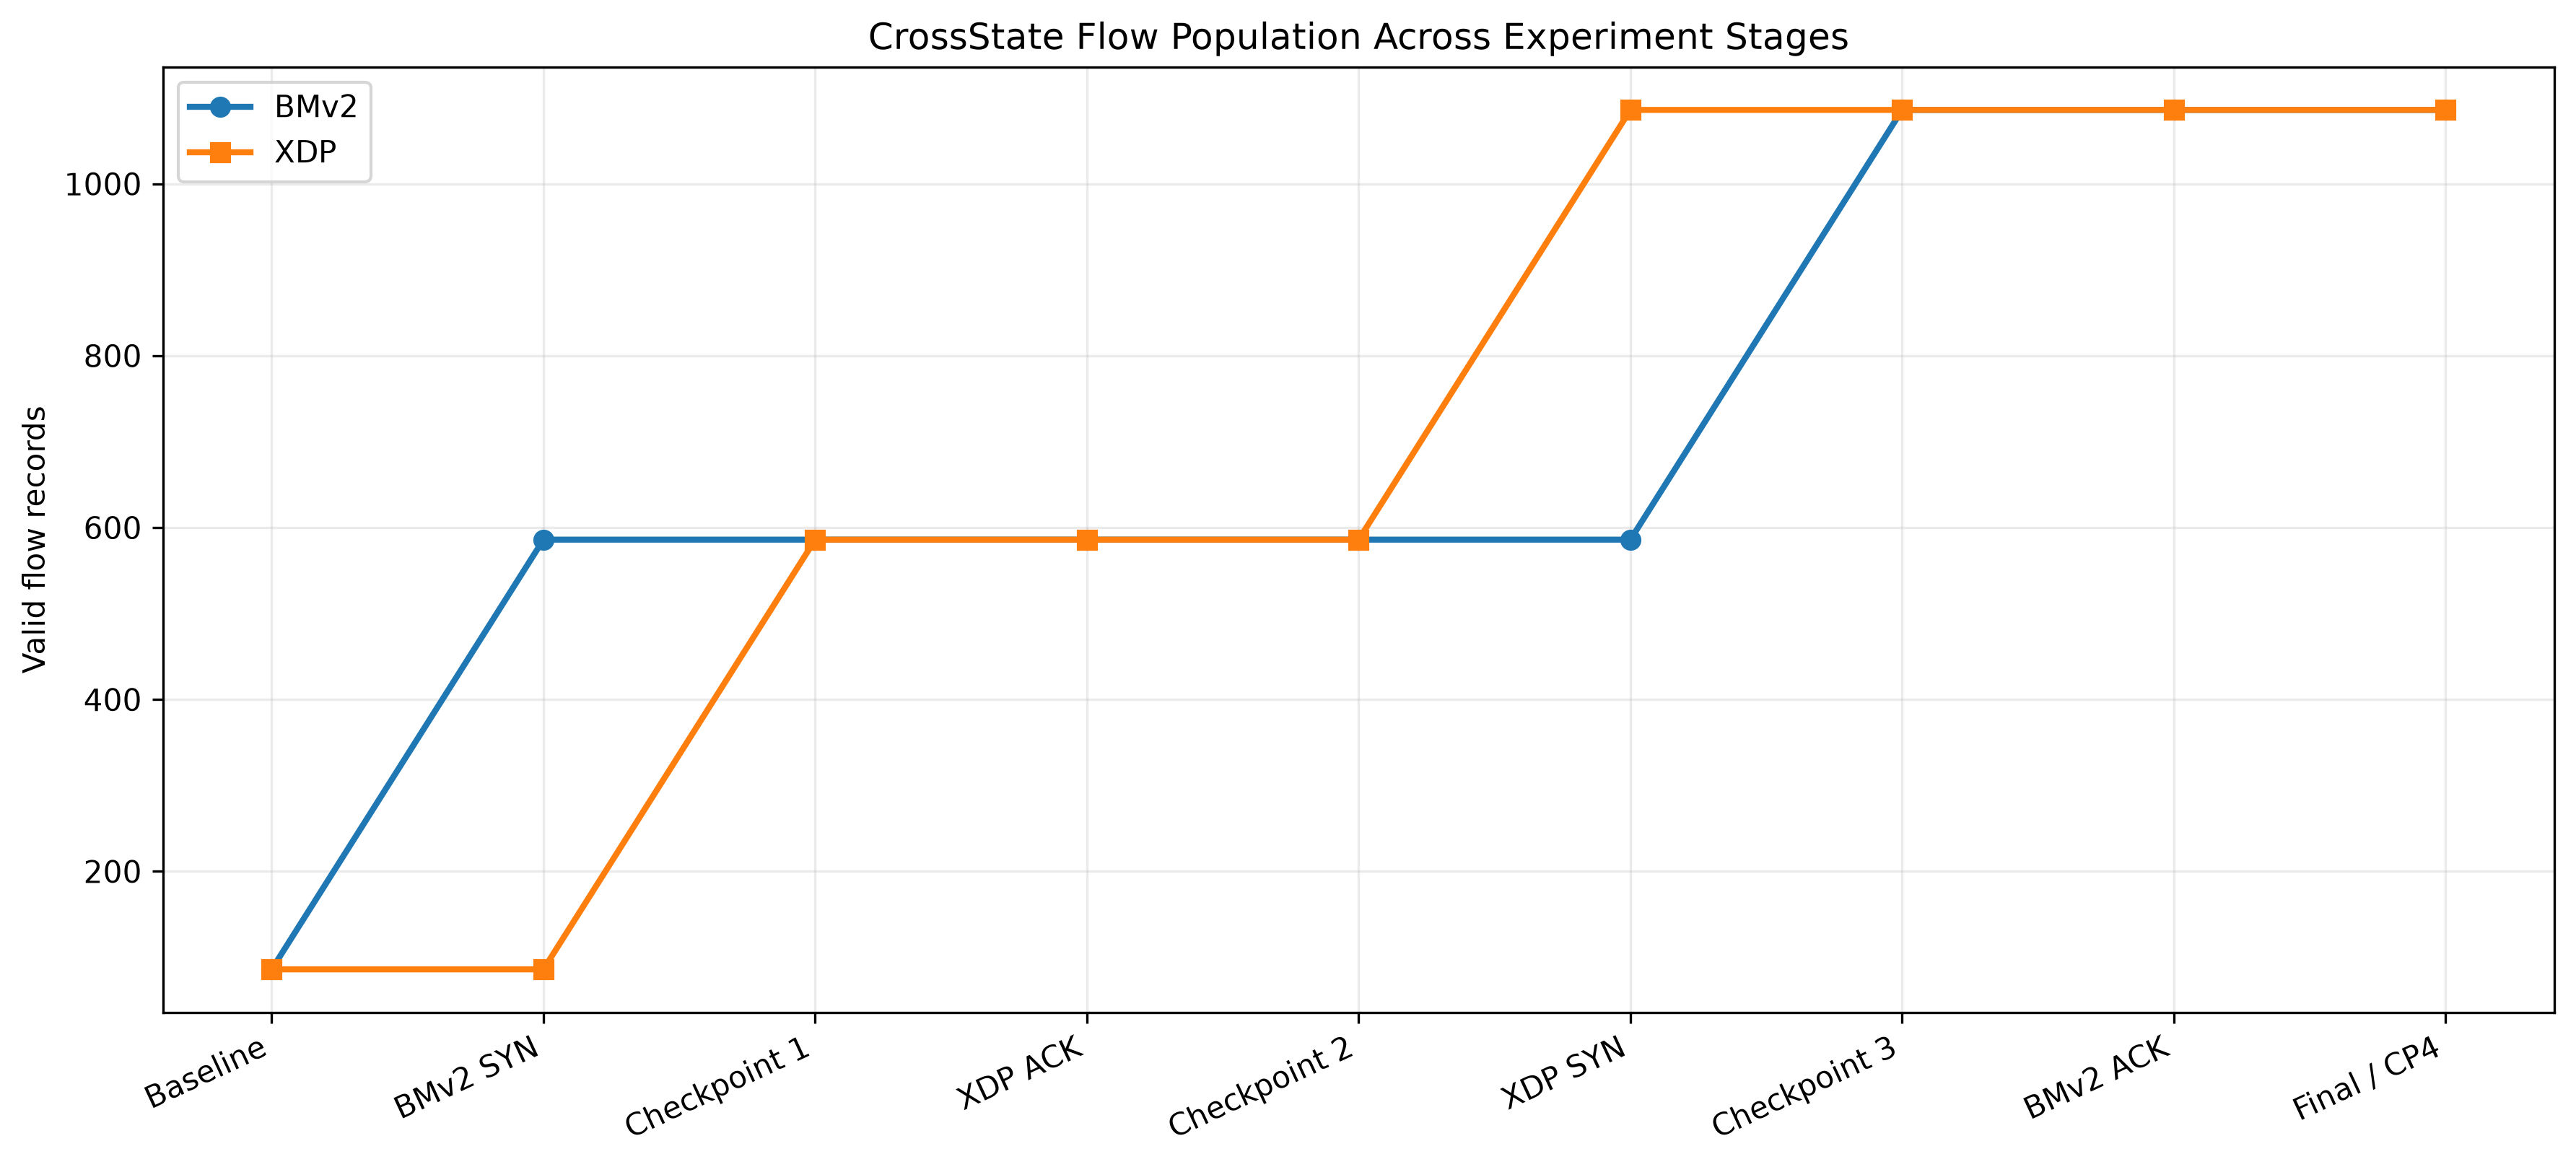
\includegraphics[width=0.74\textwidth]{figs/g7_stage.png}
\caption{Valid flow records on BMv2 and XDP across the stages of the synthetic scale test (E1).}
\label{fig:stage}
\end{figure*}

\begin{table}[!t]
\caption{Final State Equivalence and Checkpoints}
\label{tab:equiv}
\centering\footnotesize
\setlength{\tabcolsep}{2.5pt}
\begin{tabular}{@{}lrrrrr@{}}
\toprule
\textbf{Exp.} & \textbf{BMv2} & \textbf{XDP} & \textbf{Exact} & \textbf{Diff./one-sided} & \textbf{Ckpts}\\
\midrule
E1 & 1{,}086 & 1{,}086 & 1{,}086 & 0 / 0 & 4/4\\
E2 & 1{,}086 & 1{,}086 & 1{,}086 & 0 / 0 & 4/4\\
E3 & 106 & 106 & 106 & 0 / 0 & 4/4\\
\bottomrule
\end{tabular}
\end{table}

\subsection{RQ2: What Happens Without Migration}
Fig.~\ref{fig:base} and Table~\ref{tab:base} show the baseline. SYN packets are allowed in both cases because they create state. After cutover, however, an empty destination treats every follow-up packet as unsolicited: 17{,}890 of the 17{,}944 follow-up packets (99.7\%) are dropped and 996 of the 1{,}000 flows are disrupted. With \sys, no packet is dropped and no flow disrupted. The small number of follow-up packets that are allowed without migration (54, all in the last phase) are consistent with the policy re-creating state on an inside SYN; we did not trace them individually. This confirms that the state moved by \sys\ is not redundant: without it, essentially every established connection is cut at cutover.

\begin{figure}[!t]
\centering
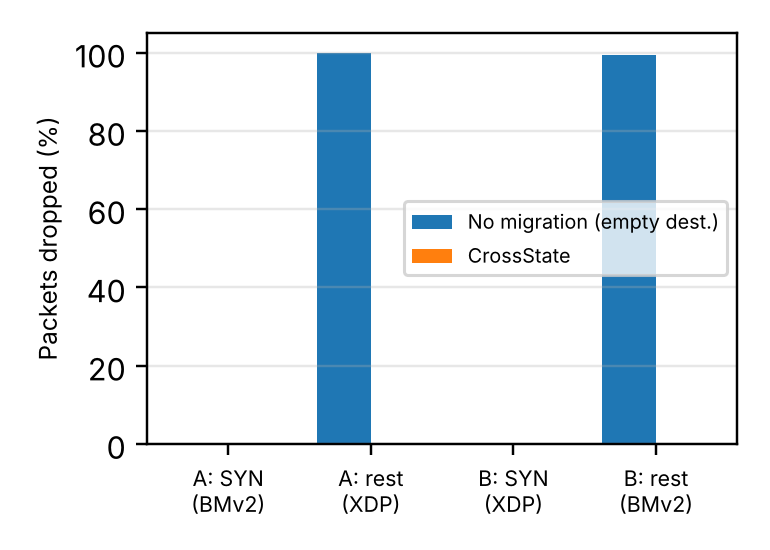
\includegraphics[width=\columnwidth]{figs/baseline_drop.png}
\caption{Packets dropped per phase with and without state migration (E2 packets replayed through the reference model).}
\label{fig:base}
\end{figure}

\begin{table}[!t]
\caption{No-Migration Baseline vs.\ \sys\ (18{,}944 Packets)}
\label{tab:base}
\centering\footnotesize
\setlength{\tabcolsep}{3pt}
\begin{tabular}{@{}lrrr@{}}
\toprule
\textbf{Metric} & \textbf{Packets} & \textbf{No migration} & \textbf{\sys}\\
\midrule
Follow-up dropped & 17{,}944 & 17{,}890 (99.7\%) & 0\\
SYN dropped & 1{,}000 & 0 & 0\\
Flows disrupted & 1{,}000 & 996 & 0\\
\bottomrule
\end{tabular}
\end{table}

\subsection{RQ3: Capacity and Collisions}
The table is direct-mapped: under the reject policy a new flow whose slot is occupied by a live different flow is dropped. Fig.~\ref{fig:coll} shows the measured rejection rate against load, together with the random-hashing expectation $1-N(1-e^{-n/N})/n$; the CRC32 mapping tracks the analytic curve closely. Rejection is 0.85\% at 1{,}000 flows, 3.7\% at 5{,}000, 7.2\% at 10{,}000, 25\% at 40{,}000 and 36.8\% when $n=N$. This also explains the 23 rejections during MAWI selection (about 2\% at 1{,}086 occupied slots). Since the migration itself is exact, this is a property of the table design, not of the migration, but it bounds the usable flow count: with $N=65{,}536$ and an acceptable rejection rate of 1\%, the table holds roughly 1{,}200 flows. The specification already reserves a bucket count, but neither datapath uses it, so bucketed collision handling is the natural next step.

\begin{figure}[!t]
\centering
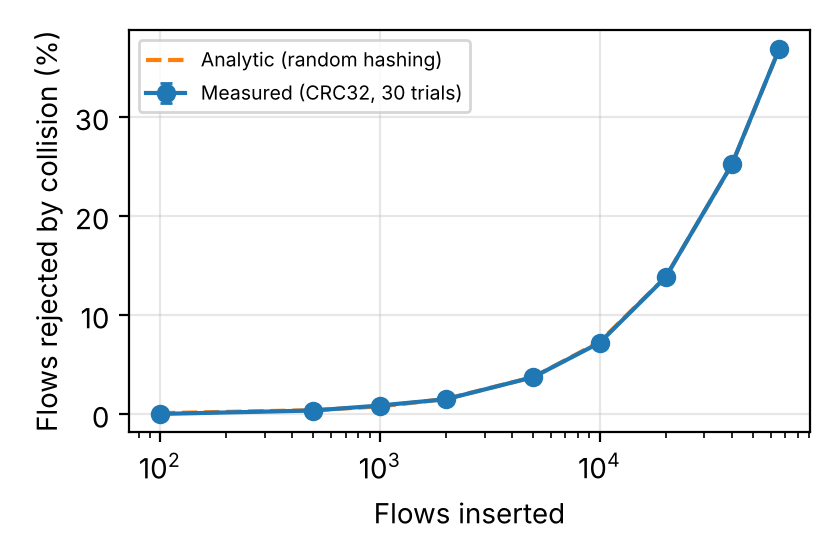
\includegraphics[width=0.95\columnwidth]{figs/collision_load.png}
\caption{Flows rejected by hash collision versus load (mean $\pm$ s.d.\ over 30 trials) and the analytic random-hashing curve.}
\label{fig:coll}
\end{figure}

\subsection{RQ4: Checkpoint Cost}
\textbf{Records written.} The tool classifies each record as insert, update or no-op and writes only changed ones. In E2 each checkpoint wrote exactly 500 records (inserts at checkpoints 1 and 3, updates at 2 and 4) and treated the rest as no-ops. Rewriting every source record would instead write 586, 586, 1{,}086 and 1{,}086 records, i.e.\ 3{,}344 in total against 2{,}000, a 40\% reduction that grows with table size (Fig.~\ref{fig:delta}).

\begin{figure}[!t]
\centering
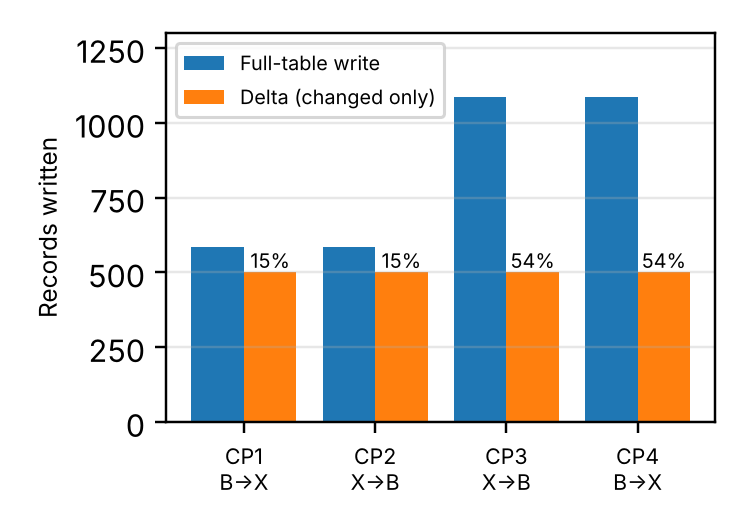
\includegraphics[width=0.92\columnwidth]{figs/delta_full.png}
\caption{Records written per checkpoint: changed-only (as implemented) versus rewriting the full table (counterfactual).}
\label{fig:delta}
\end{figure}

\textbf{Elapsed time.} Checkpoints took 47.7, 201.5, 484.1 and 130.5~s in E2 (863.8~s total) and 7.7, 13.2, 11.4 and 7.8~s for the 20-flow subset E3 (40.1~s). Normalised by the 500 records written, the elapsed time per record is 0.10, 0.40, 0.97 and 0.26~s (Fig.~\ref{fig:time}); checkpoints whose destination is BMv2 are slower than those whose destination is XDP. The code explains the direction: BMv2 import issues one command-line subprocess per record with about eleven register writes plus a read-back, whereas XDP writes go through \texttt{bpftool}. These figures are elapsed times of the whole tool run, including repeated exports and verification, so they are harness cost rather than data-plane latency, and they were measured once per configuration.

\begin{figure}[!t]
\centering
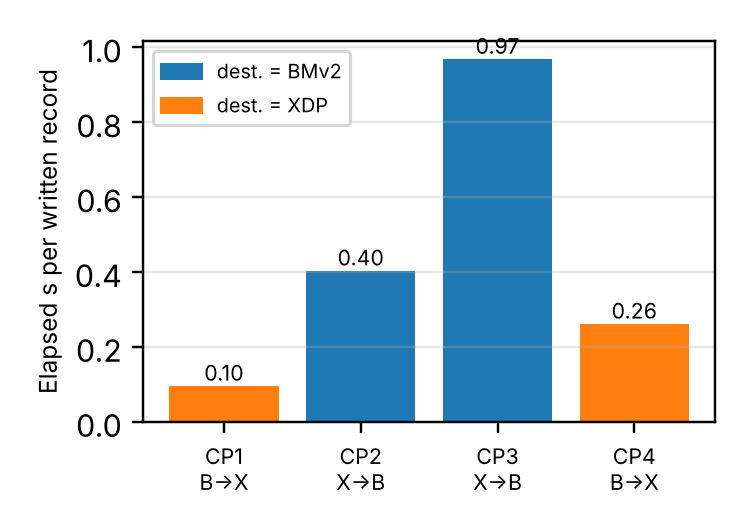
\includegraphics[width=0.92\columnwidth]{figs/time_per_record.png}
\caption{Elapsed seconds per written record for the four E2 checkpoints, by destination target.}
\label{fig:time}
\end{figure}

\subsection{RQ5: Assurance Mechanisms}
Table~\ref{tab:ladder} shows the layers that agree with the reference model. The checkpoint mechanisms (readiness gate, read-back, rollback, stability check) were exercised on every passing checkpoint: all 12 checkpoints in E1--E3 had a stable source and reached the ready state, and the 19 earlier development checkpoints (83--86 records) were also equivalent. The project's own validation notes record that an interrupted or partial import was not injected, so the \emph{negative} behaviour of these mechanisms (that a bad transfer is detected and the gate stays closed) is supported by design and unit tests but not yet by a live fault-injection experiment.

%==========================================================
\section{Discussion and Threats to Validity}
\textbf{Answers to the research questions.} RQ1: exact equivalence and 100\% decision agreement in all runs. RQ2: without migration nearly all follow-up traffic is dropped. RQ3: the direct-mapped table limits capacity to about a thousand flows at 1\% rejection. RQ4: only changed records are written, but elapsed time is dominated by the control-plane path, especially on BMv2. RQ5: assurance mechanisms are in place and pass, but live fault injection remains to be done.

\textbf{Quiesced, not live.} Packets arriving during a transfer, ordering across targets and loss-free cutover, which systems such as OpenNF treat explicitly, are not addressed. Quiescence keeps Proposition~1 simple, and the correctness criteria studied by Patowary et al.\ \cite{patowary} would apply to a live extension.

\textbf{Internal validity.} The no-migration baseline is a model replay. Timing results are single runs. The collision study uses random keys rather than MAWI keys at larger scale. BMv2 register reads are not atomic, and stability checking reduces but does not formally remove the risk of a torn snapshot if traffic is not truly quiesced.

\textbf{External validity.} Both targets are software on one host, the XDP program runs in test-echo mode, and the 1{,}000 MAWI flows are about 1.6\% of the 63{,}295 candidates tracked, so they are not a statistically representative sample of the trace.

\textbf{Planned extensions.} (i) Flow-count sweeps from 100 to 50{,}000 with per-phase timing (export, compare, import, verify); (ii) live fault injection (interrupted import, corrupted record, mutated source); (iii) repeated runs with confidence intervals; (iv) bucketed slots to raise capacity; (v) native hardware targets and enforced XDP drops.

%==========================================================
\section{Conclusion}
\sys\ migrates TCP connection-tracking state between a P4/BMv2 and an eBPF/XDP firewall in both directions using one logical schema and a verified, audited, quiesced protocol. Over four alternating migrations of 1{,}000 real MAWI flows, all checkpoints passed, all 18{,}944 decisions matched the reference model, and the 1{,}086-record tables were identical; the same packets without migration lose 99.7\% of follow-up traffic. The study also quantifies the limits of the current design: a direct-mapped table that rejects 7.2\% of new flows at 10{,}000 flows, and checkpoint times dominated by the BMv2 control path. Future work targets live migration, higher capacity and native hardware.

\section*{Acknowledgment}
The authors thank their supervisor, Dr.\ Jagadeesha R.\ Bhatt, for guidance throughout this project. The MAWI trace is courtesy of the WIDE Project.

%==========================================================
\begin{thebibliography}{99}\small
\bibitem{p4} P.~Bosshart \emph{et al.}, ``P4: Programming protocol-independent packet processors,'' \emph{ACM SIGCOMM Comput.\ Commun.\ Rev.}, vol.~44, no.~3, pp.~87--95, 2014.
\bibitem{xdp} T.~H{\o}iland-J{\o}rgensen \emph{et al.}, ``The eXpress Data Path: Fast programmable packet processing in the operating system kernel,'' in \emph{Proc.\ ACM CoNEXT}, 2018, pp.~54--66.
\bibitem{smartnic} E.~F.~Kfoury, S.~Choueiri, A.~Mazloum, A.~AlSabeh, J.~Gomez, and J.~Crichigno, ``A comprehensive survey on SmartNICs: Architectures, development models, applications, and research directions,'' \emph{IEEE Access}, vol.~12, pp.~107297--107336, 2024.
\bibitem{p4sec} G.~Singh, H.~B.~Acharya, and M.~Kwon, ``Programmable data planes for network security,'' arXiv:2507.22165, 2025.
\bibitem{cofilter} J.~Cao, J.~Bi, Y.~Zhou, and C.~Zhang, ``CoFilter: A high-performance switch-assisted stateful packet filter,'' in \emph{Proc.\ ACM SIGCOMM Posters and Demos}, 2018, pp.~9--11.
\bibitem{rapid} Y.~Feng \emph{et al.}, ``Empower programmable pipeline for advanced stateful packet processing,'' in \emph{Proc.\ USENIX NSDI}, 2024.
\bibitem{ebpfp4} M.~Simon, H.~Stubbe, S.~Gallenm{\"u}ller, and G.~Carle, ``Honey for the ice bear -- Dynamic eBPF in P4,'' in \emph{Proc.\ Workshop on eBPF and Kernel Extensions (eBPF '24)}, Sydney, Australia, 2024, doi:10.1145/3672197.3673436.
\bibitem{bmv2} P4 Language Consortium, ``Behavioral Model (BMv2),'' GitHub repository, \url{https://github.com/p4lang/behavioral-model}.
\bibitem{opennf} A.~Gember-Jacobson \emph{et al.}, ``OpenNF: Enabling innovation in network function control,'' in \emph{Proc.\ ACM SIGCOMM}, 2014, pp.~163--174.
\bibitem{splitmerge} S.~Rajagopalan \emph{et al.}, ``Split/Merge: System support for elastic execution in virtual middleboxes,'' in \emph{Proc.\ USENIX NSDI}, 2013, pp.~227--240.
\bibitem{swing} S.~Luo \emph{et al.}, ``Swing State: Consistent updates for stateful and programmable data planes,'' in \emph{Proc.\ ACM SOSR}, 2017.
\bibitem{redplane} D.~Kim, J.~Nelson, D.~R.~K.~Ports, V.~Sekar, and S.~Seshan, ``RedPlane: Enabling fault-tolerant stateful in-switch applications,'' in \emph{Proc.\ ACM SIGCOMM}, 2021.
\bibitem{cora} S.~Xi \emph{et al.}, ``Cora: Accelerating stateful network applications with SmartNICs,'' arXiv:2410.22229, 2024.
\bibitem{switchnic} Y.~Lei, F.~Pereira, A.~Krishnamurthy, and J.~Sherry, ``SwitchNIC: An hybrid architecture for network functions with fast and consistent shared state,'' \emph{Proc.\ ACM Netw.}, vol.~3, no.~CoNEXT4, art.~46, Dec.\ 2025, doi:10.1145/3768993.
\bibitem{patowary} R.~Patowary, G.~Barua, and R.~Sukapuram, ``Correctness of flow migration across network function instances,'' arXiv:2404.07701, 2024.
\bibitem{mafaf} N.~Salah, A.~El-Sayed, and O.~M.~Elkomy, ``MAFAF: Mobility-aware flow anchoring and dynamic state migration in edge SDN using P4,'' \emph{Int.\ J.\ Comput.\ Informat.\ (Zagazig Univ.)}, vol.~9, pp.~74--93, Dec.\ 2025.
\bibitem{mawi} K.~Cho, K.~Mitsuya, and A.~Kato, ``Traffic data repository at the WIDE project,'' in \emph{Proc.\ USENIX Annual Technical Conf.\ (FREENIX Track)}, 2000; MAWI Working Group Traffic Archive, \url{http://mawi.wide.ad.jp/mawi/}.
\end{thebibliography}
\end{document}
